\thispagestyle{duongvaotoanhocnone}
\pagestyle{duongvaotoanhoc}
\everymath{\color{duongvaotoanhoc}}
\graphicspath{{../duongvaotoanhoc/pic/}}
\blfootnote{$^1$\color{duongvaotoanhoc}Theo Quanta Magazine.}
\blfootnote{$^2$\color{duongvaotoanhoc}Hà Nội.}
\begingroup
\AddToShipoutPicture*{\put(0,616){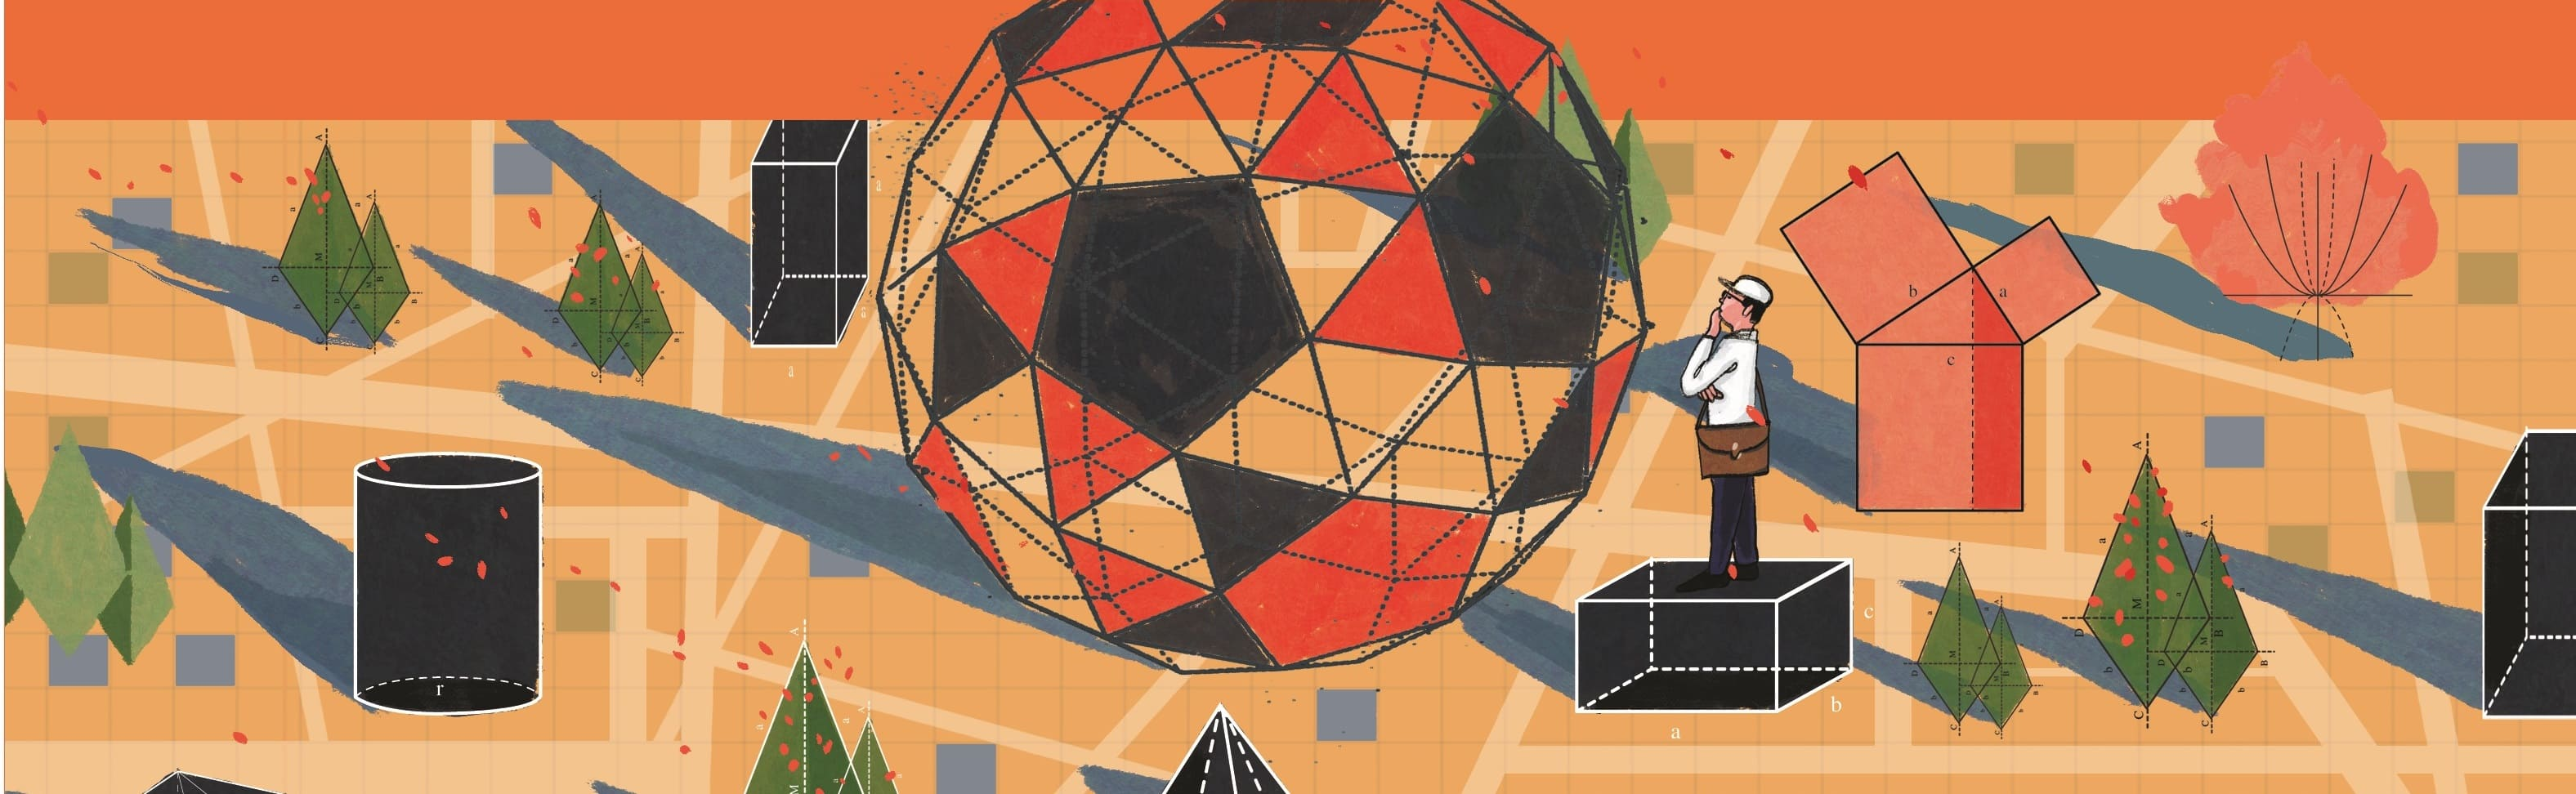
\includegraphics[width=19.3cm]{../bannerduongvao}}}
\AddToShipoutPicture*{\put(136,508){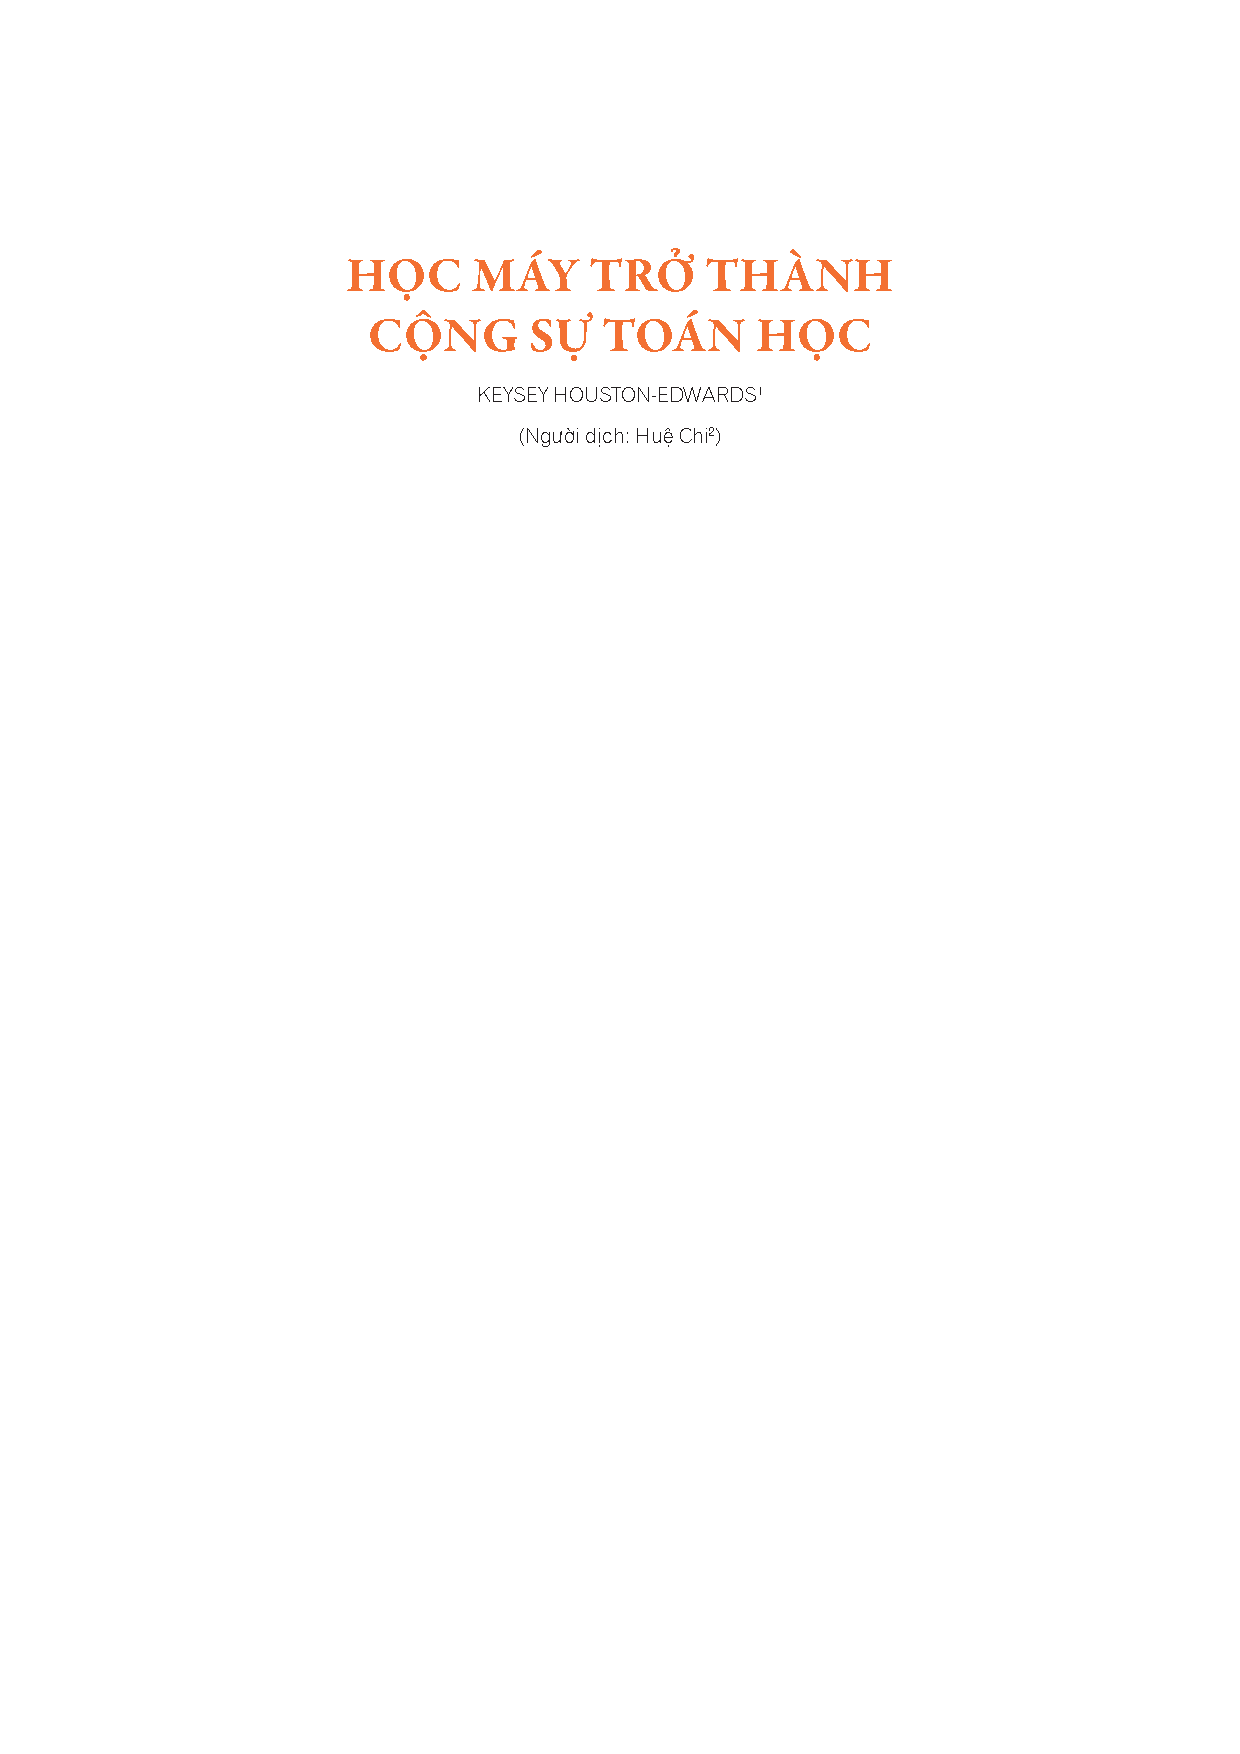
\includegraphics[scale=1]{../tieude1.pdf}}}
\centering
\endgroup

\vspace*{200pt}

\begin{multicols}{2}	
	\textit{Hai hợp tác gần đây giữa các nhà toán học và công ty DeepMind đã cho thấy tiềm năng của học máy trong việc giúp các nhà nghiên cứu đưa ra các giả thuyết mới trong toán học.}
	\begin{figure}[H]
		\centering
		\vspace*{-5pt}
		\captionsetup{labelformat= empty, justification=centering}
		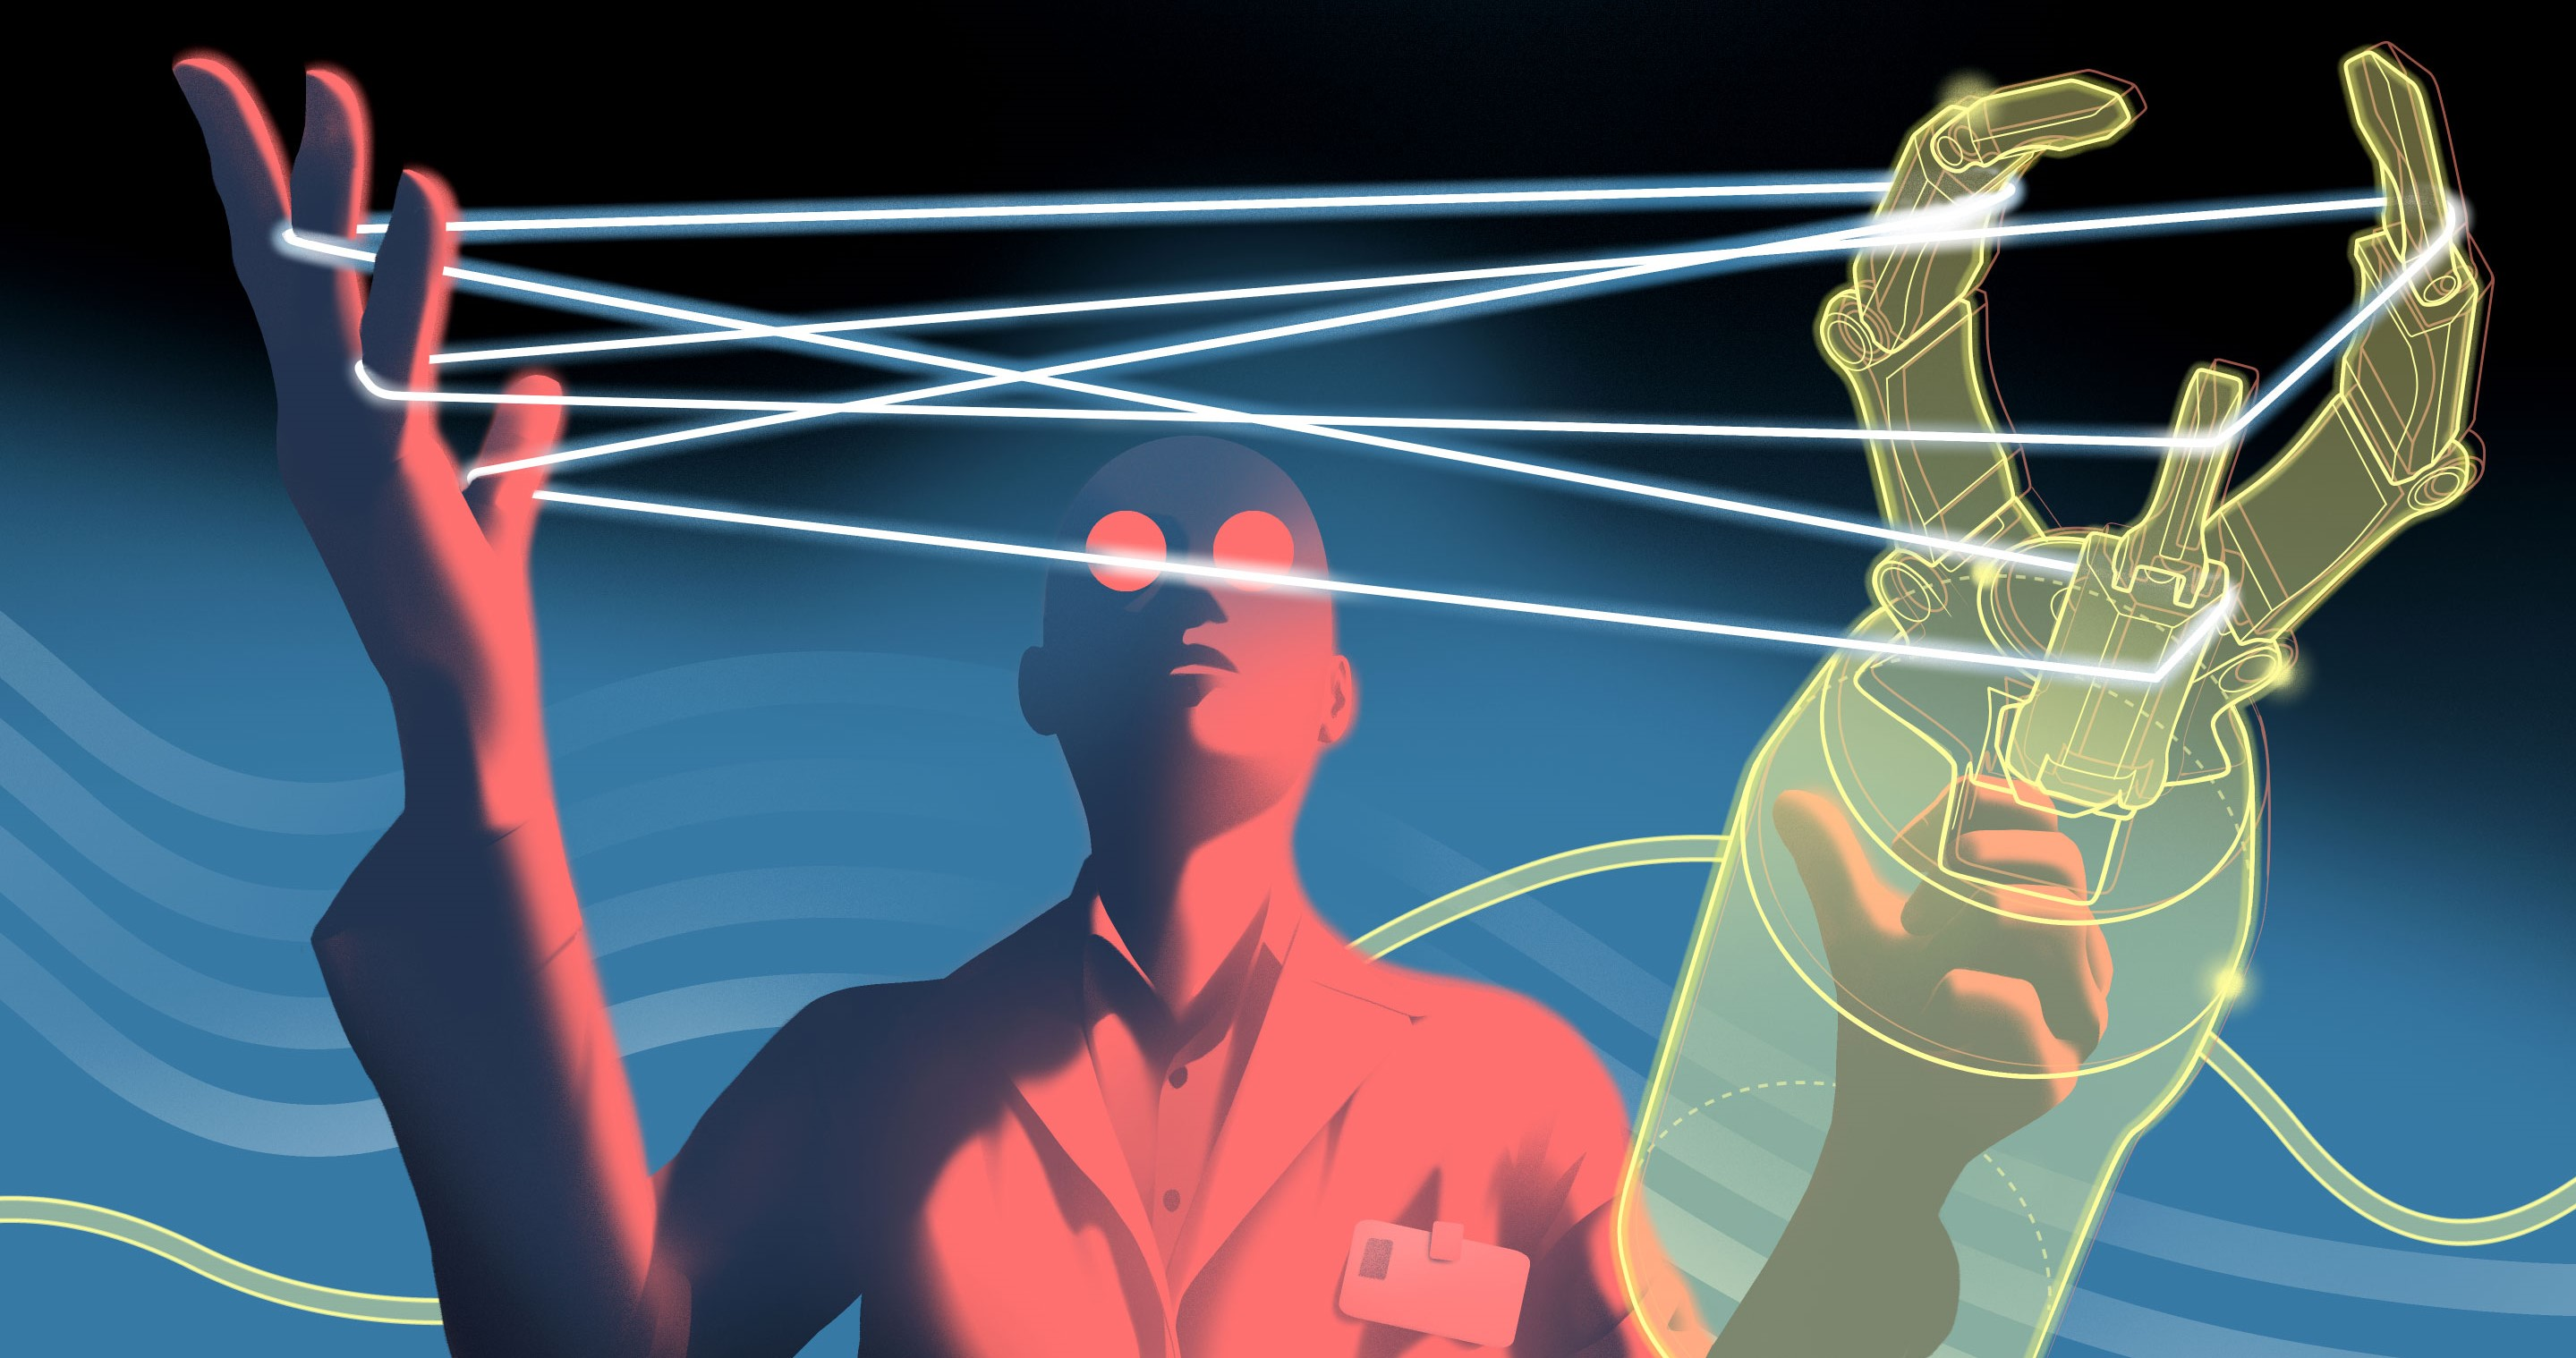
\includegraphics[width=1\linewidth]{1}
		%		\caption{\small\textit{\color{duongvaotoanhoc}Señor Salme, Quanta magazine.}}
		\vspace*{-15pt}
	\end{figure}
	Các nhà toán học thường làm việc cùng nhau khi muốn tìm kiếm những cái nhìn sâu sắc về một vấn đề khó. Đó là một kiểu quy trình cộng tác có vẻ như đòi hỏi hoàn toàn sự trao đổi giữa người và người.
	\vskip 0.05cm
	Nhưng trong hai kết quả mới đây, máy móc đã thay thế một phần vai trò của người cộng tác khoa học. Các bài báo của kiểu hợp tác như vậy được hoàn thành vào cuối tháng $11$ năm $2021$, và được tóm tắt trong một bài báo gần đây trên tạp chí Nature.
	\vskip 0.05cm
	Geordie Williamson, một nhà toán học của Đại học Sydney và là đồng tác giả của một trong những bài báo đó, cho biết: ``Những điều tôi yêu thích ở toán học là các khía cạnh trực giác và sáng tạo của nó. Các mô hình học máy đã hỗ trợ những điều đó theo cách mà trước đây tôi chưa từng cảm nhận được từ máy tính."
	\vskip 0.05cm
	Hai nhóm nhà toán học khác nhau đã làm việc cùng với công ty chuyên phát triển các hệ thống trí tuệ nhân tạo tiên tiến DeepMind, một công ty con của Alphabet (công ty mẹ của Google).
	\vskip 0.05cm
	András Juhász và Marc Lackenby của Đại học Oxford đã dạy các mô hình học máy của DeepMind để tìm kiếm các mẫu lặp trong các đối tượng hình học có tên gọi là \textit{nút}. Các mô hình đã phát hiện ra các kết nối mà Juhász và Lackenby xây dựng ra để liên kết hai lĩnh vực trong lý thuyết nút mà từ lâu các nhà toán học đã phỏng đoán là có liên quan với nhau. Trong một công trình khác, Williamson đã sử dụng các mô hình học máy để tinh chỉnh một giả thuyết cũ kết nối giữa đồ thị và đa thức.
	\vskip 0.05cm
	Trong nhiều năm, máy tính đã hỗ trợ nghiên cứu toán học như một công cụ trợ giúp chứng minh nhằm đảm bảo tính đúng đắn trong các bước suy luận logic của một chứng minh toán học, hoặc như một công cụ mạnh có thể xử lý một lượng lớn các dữ liệu để tìm ra các phản ví dụ cho các giả thuyết.
	\vskip 0.05cm
	Các công trình mới kể trên đại diện cho một hình thức hợp tác khác giữa con người và máy móc. Nó chỉ ra rằng bằng cách kết hợp một cách có chọn lọc học máy vào giai đoạn phát triển của nghiên cứu, các nhà toán học có thể phát hiện ra các manh mối mà có thể khó tìm thấy chúng nếu không có sự trợ giúp của máy móc.
	\vskip 0.05cm
	Radmila Sazdanovic của Đại học Bang North Carolina cho biết: ``Điều tuyệt vời nhất về các công trình này -- và nó thực sự là một bước đột phá lớn -- là tất cả các mảnh ghép khớp lại với nhau và những người này đã làm việc như một nhóm. Đó thực sự là một hợp tác liên ngành."
	\vskip 0.05cm
	Tuy nhiên, một số nhà quan sát coi những hợp tác này không phải là một cuộc cách mạng trong cách thức tiến hành nghiên cứu toán học. Trong khi máy tính hướng các nhà toán học tới một loạt các mối quan hệ có thể có thì bản thân các nhà toán học cần xác định xem những mối quan hệ nào là đáng khám phá.
	\vskip 0.05cm
	Ernest Davis, một nhà khoa học máy tính của Đại học New York, viết trong email: ``Tất cả những công việc khó khăn đều được thực hiện bởi con người -- các nhà toán học."
	\vskip 0.05cm
	\textbf{\color{duongvaotoanhoc}Các mẫu lặp trong dữ liệu}
	\vskip 0.05cm
	Học máy dự đoán kết quả đầu ra dựa vào dữ liệu đầu vào: nếu cung cấp cho nó một dữ liệu điển hình về sức khỏe thì nó sẽ đưa ra một chẩn đoán lâm sàng; nếu đưa cho nó hình ảnh của một con vật thì nó sẽ cho biết tên của loài đó.
	\vskip 0.05cm
	Điều này thường được thực hiện thông qua tiếp cận học máy có tên là học có giám sát, trong đó các nhà nghiên cứu chủ yếu dạy máy tính đưa ra dự đoán bằng cách cung cấp cho nó nhiều ví dụ.
	\vskip 0.05cm
	Chẳng hạn, hãy tưởng tượng bạn muốn dạy một mô hình học máy xác định xem một bức ảnh chụp một con mèo hay là một con chó. Đầu tiên, các nhà nghiên cứu cung cấp cho mô hình học máy nhiều ví dụ về mỗi loài. Dựa trên các dữ liệu huấn luyện đó, máy tính xây dựng một hàm toán học cực kỳ phức tạp, mà về bản chất là một cỗ máy đưa ra các dự đoán. Sau đó, một khi chức năng dự đoán đã được thiết lập, các nhà nghiên cứu đưa ra một bức ảnh mới cho mô hình và nó sẽ trả lời đó là mèo hay chó với xác suất tương ứng.
	\begin{figure}[H]
		\centering
		\vspace*{-5pt}
		\captionsetup{labelformat= empty, justification=centering}
		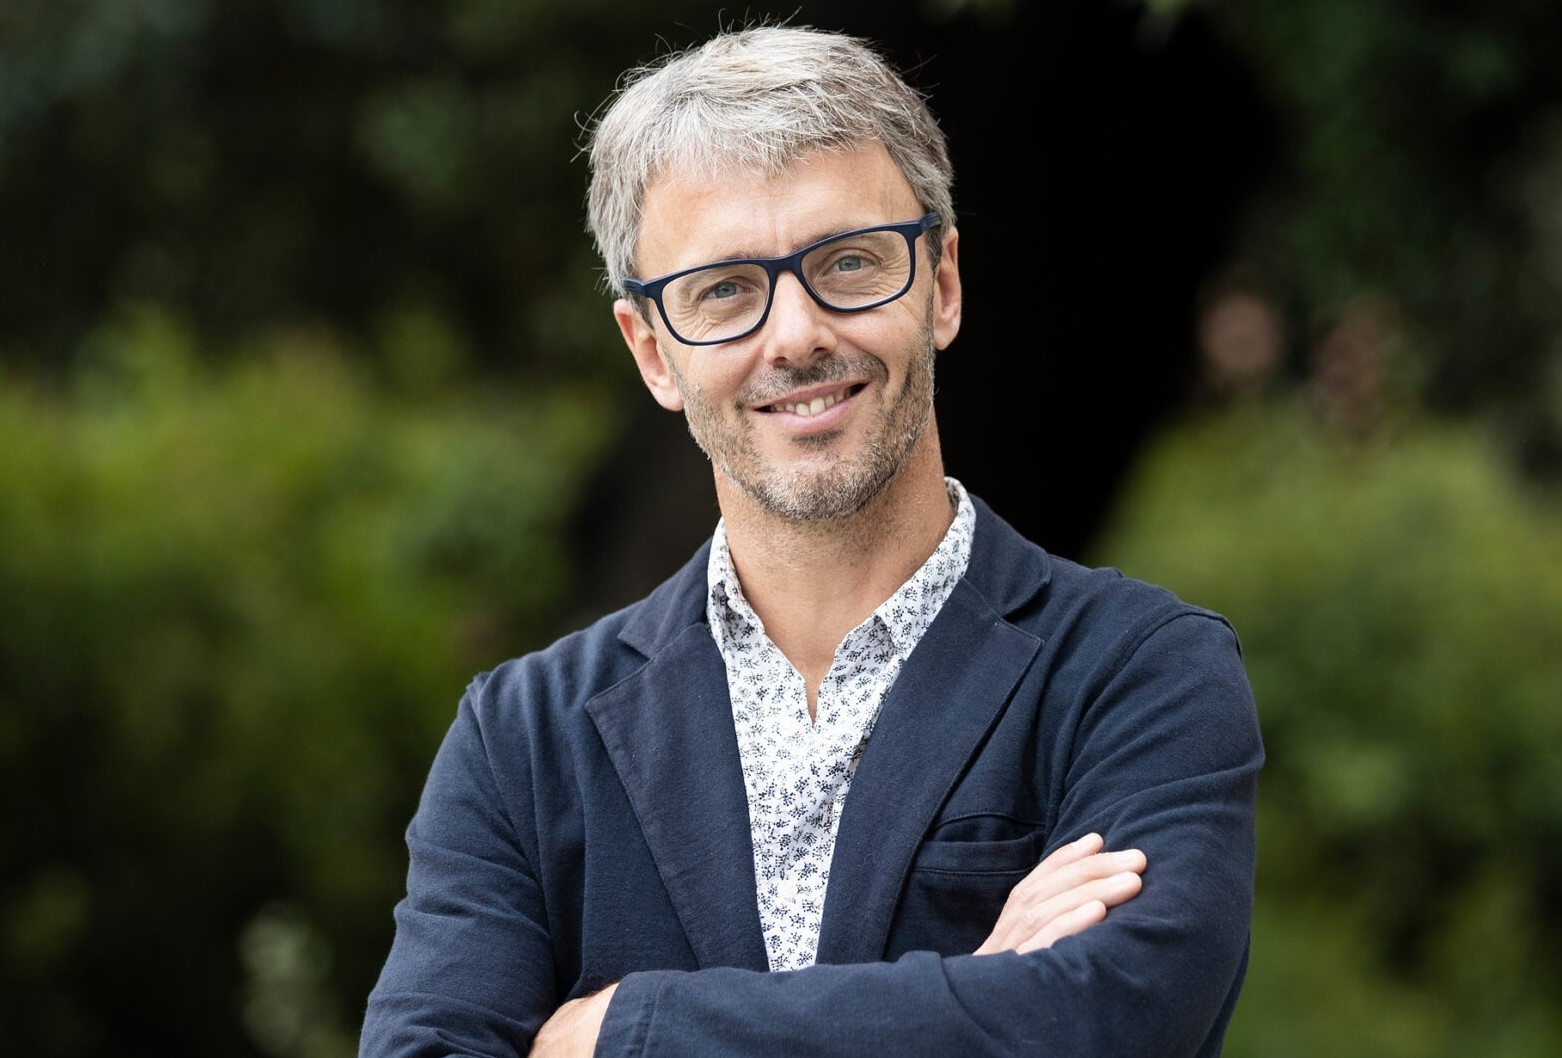
\includegraphics[width=1\linewidth]{2}
		\caption{\small\textit{\color{duongvaotoanhoc}Geordie Williamson của Đại học Sydney đã giúp DeepMind xác định các vấn đề toán học phù hợp với học máy.}}
		\vspace*{-10pt}
	\end{figure}
	Để khiến việc học có giám sát trở thành một công cụ nghiên cứu hữu ích, các nhà toán học phải tìm ra những câu hỏi phù hợp để DeepMind giải quyết. Họ cần các bài toán liên quan đến các đối tượng toán học mà ở đó có sẵn nhiều dữ liệu huấn luyện -- một tiêu chí mà nhiều vấn đề toán học không đáp ứng được.
	\vskip 0.05cm
	Họ cũng cần tìm cách tận dụng khả năng mạnh mẽ của DeepMind trong việc phát hiện các mối liên hệ tiềm ẩn, đồng thời khắc phục những hạn chế đáng kể của nó với vai trò là cộng tác viên khoa học. Thông thường, mô hình học máy hoạt động như một hộp đen, tạo ra kết quả đầu ra từ các dữ liệu đầu vào theo các quy tắc mà con người không thể giải mã được.
	\vskip 0.05cm
	Alex Davies, một nhà nghiên cứu tại DeepMind, cho biết: ``[Máy tính] có thể nhìn thấy những điều bất thường, nhưng cũng phải vật lộn để giải thích một cách hiệu quả."
	\vskip 0.05cm
	Các nhà toán học không tìm đến DeepMind chỉ để có các câu trả lời đúng. Để thực sự có những tiến bộ khoa học, họ cần biết lý do vì sao lại có các mối liên hệ – bước mà máy tính không thể làm được.
	\vskip 0.05cm
	\textbf{\color{duongvaotoanhoc}Kết nối các bất biến}
	\vskip 0.05cm
	Năm $2018$, Williamson và Demis Hassabis, giám đốc điều hành và đồng sáng lập của DeepMind, cùng được bầu làm thành viên của Hội Khoa học Hoàng gia Anh (Royal Society), một tổ chức gồm các nhà khoa học xuất sắc của Anh. Trong  giờ nghỉ giải lao tại buổi lễ kết nạp, họ nhận thấy có những mối quan tâm chung.
	\vskip 0.05cm
	Williamson nói: ``Tôi đã suy nghĩ một chút ít về cách học máy có thể giúp ích cho toán học và anh ấy đã suy nghĩ rất nhiều về điều đó. Kiểu như chúng tôi nảy ra những ý tưởng từ nhau."
	\vskip 0.05cm
	Họ quyết định rằng một chuyên ngành toán học được gọi là lý thuyết nút sẽ là nền tảng thử nghiệm lý tưởng cho sự hợp tác giữa con người và máy tính. Nó liên quan đến các đối tượng toán học có tên gọi là nút, mà bạn có thể coi như những vòng dây chằng chịt. Lý thuyết nút phù hợp với các yêu cầu đối với học máy vì nó có dữ liệu phong phú -- có hàng triệu nút tương đối đơn giản -- và vì nhiều thuộc tính của nút thắt có thể được tính toán dễ dàng bằng phần mềm hiện có.
	\vskip 0.05cm
	Williamson đề nghị DeepMind liên hệ với Lackenby, một nhà lý thuyết nút có tiếng, để tìm ra một vấn đề toán học cụ thể để giải quyết.
	\vskip 0.05cm	
	Juhász và Lackenby hiểu rõ điểm mạnh và điểm yếu của học máy. Với những thứ đó, họ hy vọng sẽ sử dụng nó để tìm ra những mối liên hệ mới giữa các loại bất biến khác nhau, những thuộc tính được sử dụng để phân biệt các nút với nhau.
	\vskip 0.05cm
	Hai nút được coi là khác nhau khi không thể tháo gỡ chúng (mà không cắt chúng) để chúng trông giống nhau. Bất biến là các thuộc tính bản chất của nút, không thay đổi trong quá trình tháo gỡ (do đó có tên là ``bất biến"). Vì vậy, nếu hai nút có một bất biến nhận các giá trị khác nhau, thì không thể thao tác để chúng trở nên giống nhau.
	\begin{figure}[H]
		\centering
		\vspace*{-5pt}
		\captionsetup{labelformat= empty, justification=centering}
		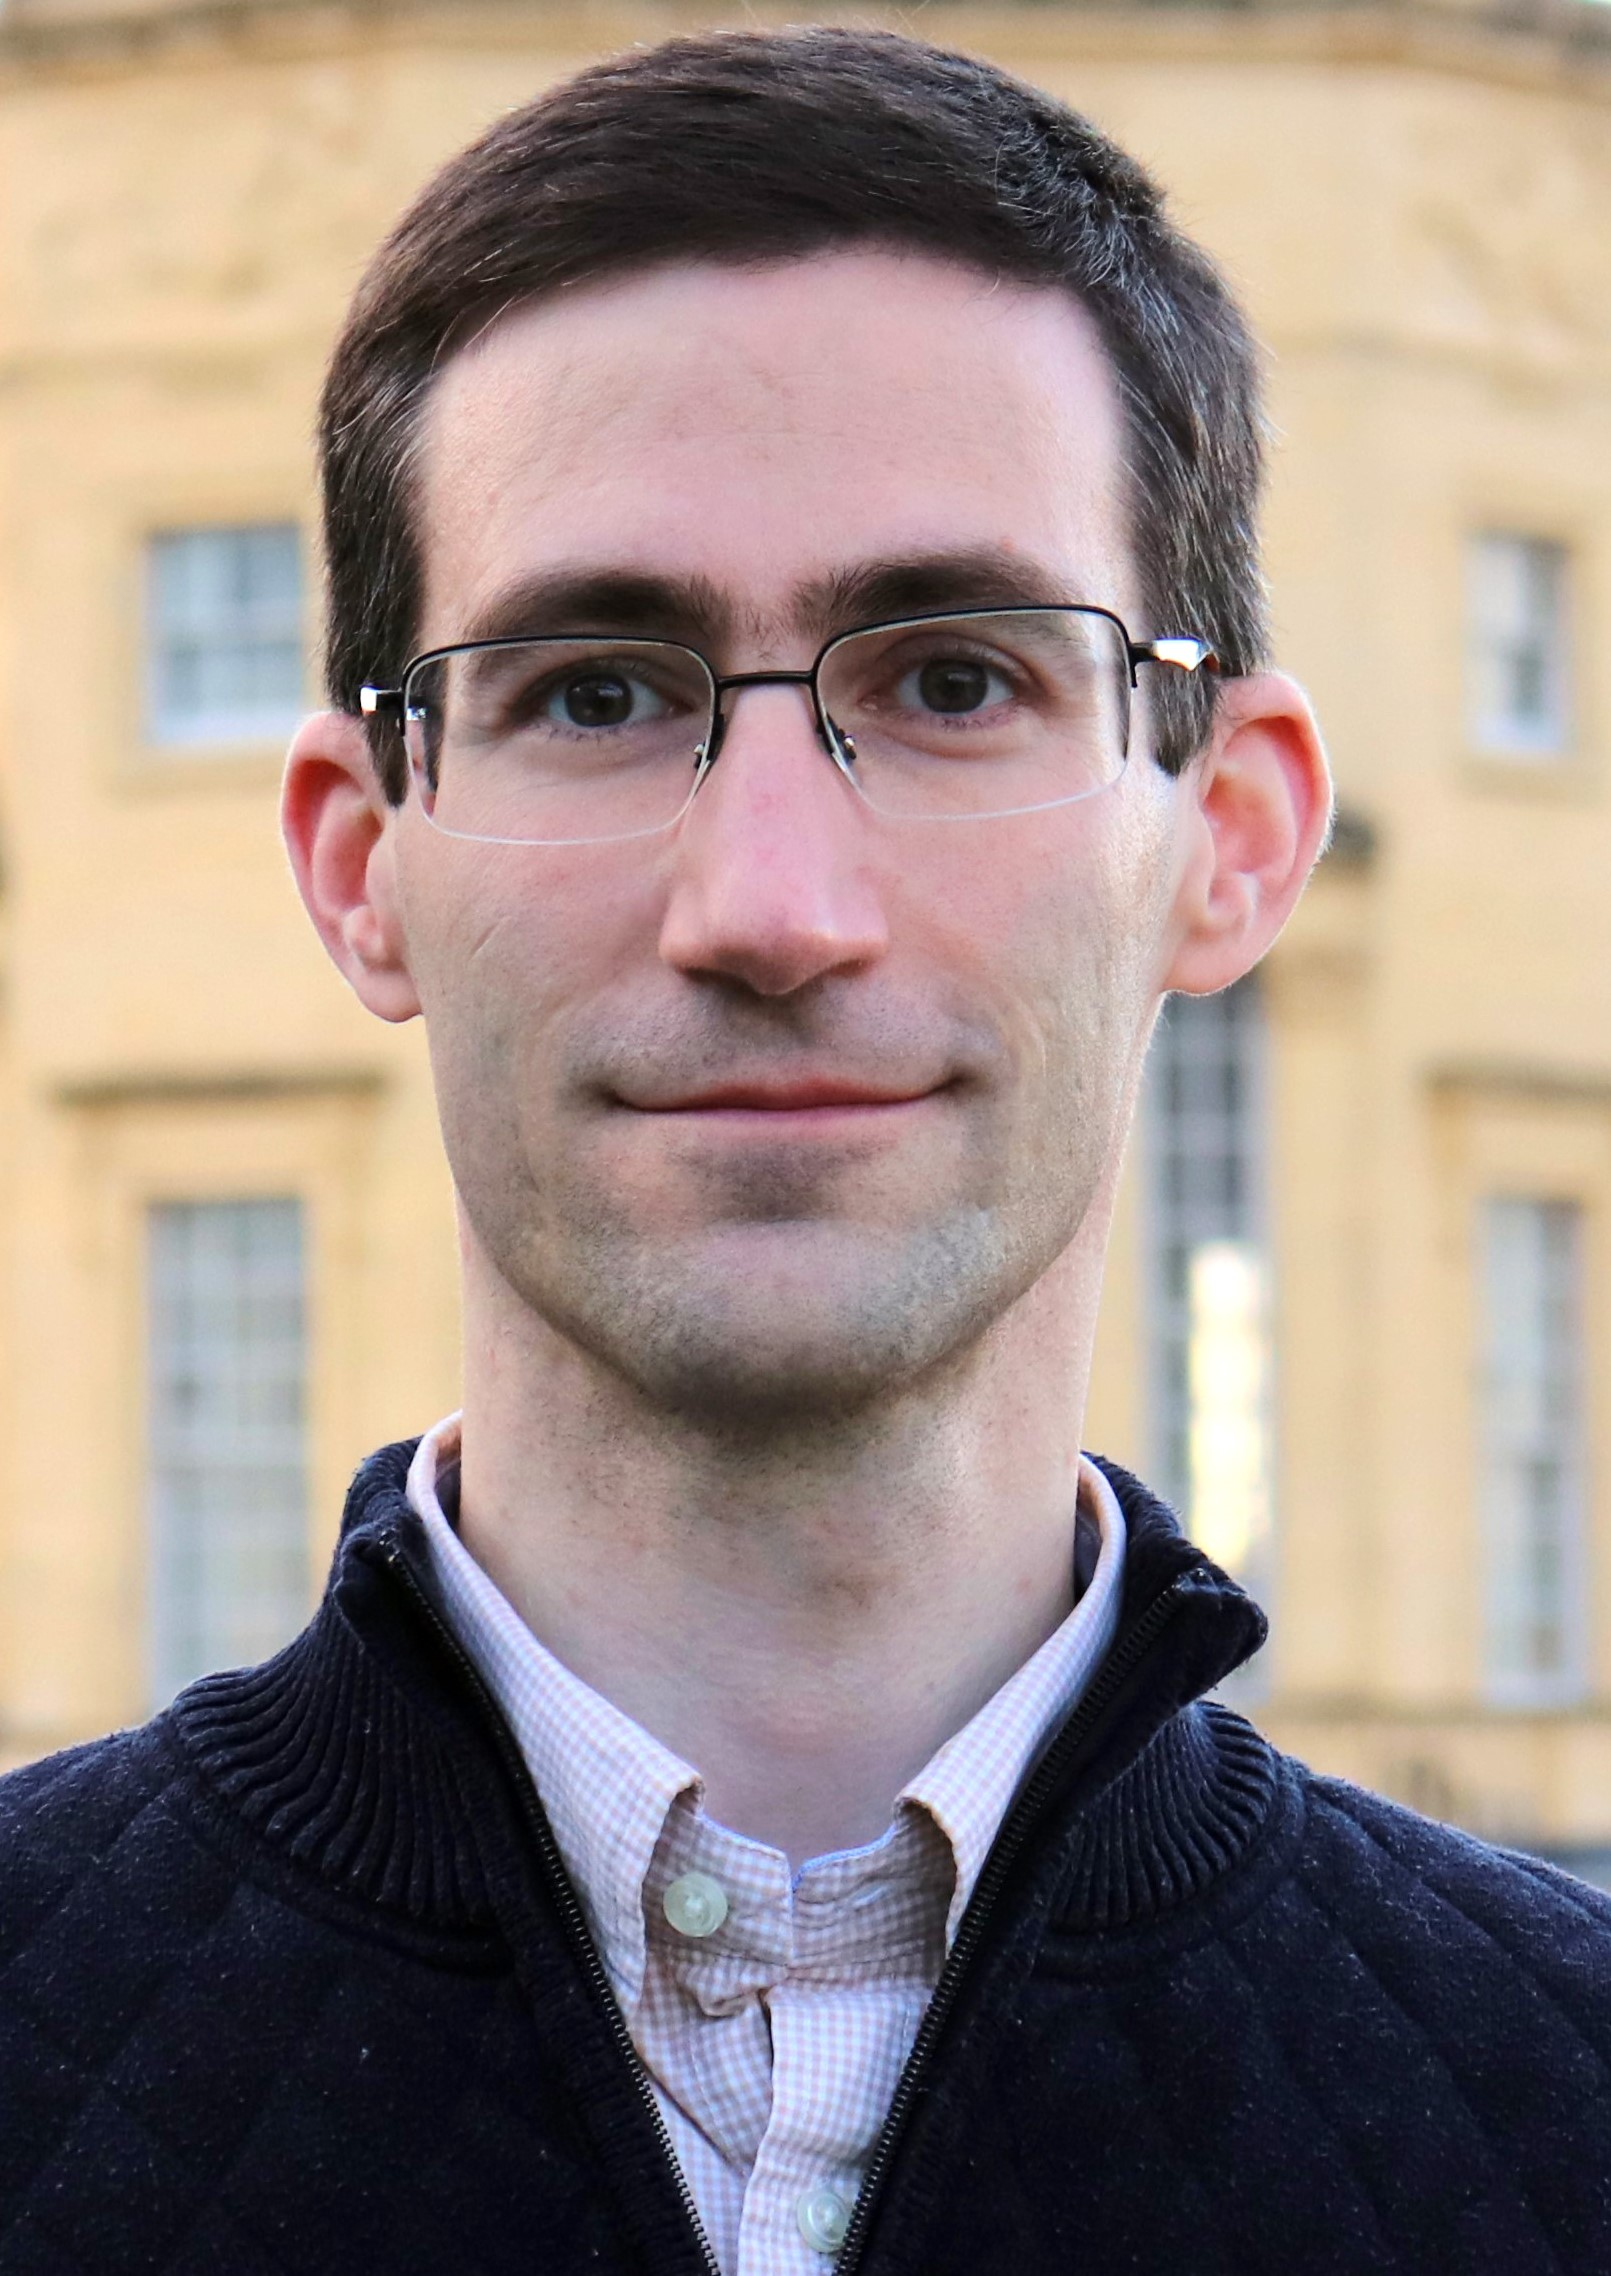
\includegraphics[height=0.425\linewidth]{3}
		
\includegraphics[height=0.425\linewidth]{4}
		\caption{\small\textit{\color{duongvaotoanhoc}András Juhász và Marc Lackenby của Đại học Oxford đã chọn lọc  một tập hợp các manh mối được tạo ra nhờ học máy để xác định một công thức phiên dịch giữa các bất biến nút thắt khác~nhau.}}
		\vspace*{-10pt}
	\end{figure}
	Có nhiều loại bất biến nút khác nhau, được đặc trưng bởi cách mà chúng mô tả các nút. Một số trong chúng mang tính hình học nhiều hơn, một số khác mang tính đại số và một số thì có tính tổ hợp. Tuy nhiên, các nhà toán học chỉ có thể thiết lập được rất ít mối quan hệ giữa các bất biến thuộc các loại khác nhau. Họ thường không biết liệu các bất biến khác nhau có thực chất đo lường cùng một đặc điểm của nút từ các góc nhìn khác nhau hay không.
	\vskip 0.05cm
	\textbf{\color{duongvaotoanhoc}Xác minh chữ ký}
	\vskip 0.05cm
	Để theo đuổi câu hỏi của Juhász và Lackenby, các nhà nghiên cứu tại DeepMind đã phát triển một bộ dữ liệu với hơn 2 triệu nút. Đối với mỗi nút, họ tính toán các bất biến khác nhau. Sau đó, họ sử dụng học máy để tìm kiếm các mẫu lặp gắn kết các bất biến với nhau. Máy tính phát hiện được nhiều mẫu, nhưng hầu hết trong số đó không quá thú vị đối với các nhà toán học.
	\vskip 0.05cm
	``Chúng tôi thấy khá nhiều mẫu lặp đã được biết đến hoặc đã được chỉ ra là không đúng," Lackenby nói. ``Là những nhà toán học, chúng tôi đã loại bỏ khá nhiều thứ mà máy tính gửi cho chúng tôi."
	\vskip 0.05cm
	Không giống như Juhász và Lackenby, hệ thống học máy không hiểu được lý thuyết toán học đằng sau. Dữ liệu đầu vào được tính toán từ các bất biến nút, nhưng máy tính chỉ nhìn thấy danh sách các con số.
	\vskip 0.05cm
	Davis cho biết: ``Về phía hệ thống học máy, các con số đó cũng giống như doanh số bán hàng của nhiều món ăn khác nhau tại cửa hàng McDonald mà thôi."
	\vskip 0.05cm
	Cuối cùng, hai nhà toán học quyết định tìm cách dạy máy tính xuất ra một bất biến đại số quan trọng được gọi là "chữ ký" của một nút chỉ dựa trên thông tin về các bất biến hình học của nút.
	\vskip 0.05cm
	Sau khi Juhász và Lackenby xác định được vấn đề, các nhà nghiên cứu tại DeepMind bắt đầu xây dựng thuật toán học máy cụ thể. Họ đã huấn luyện máy tính lấy $30$ bất biến hình học của một nút làm đầu vào và xuất ra chữ ký của nút. Thuật toán hoạt động tốt và sau một vài tuần làm việc, DeepMind có thể dự đoán chính xác chữ ký của hầu hết các nút.
	\vskip 0.05cm
	Tiếp theo, các nhà nghiên cứu cần tìm hiểu xem mô hình học máy đã đưa ra những dự đoán này như thế nào. Để làm điều đó, nhóm nghiên cứu tại DeepMind quay sang một kỹ thuật được gọi là phân tích độ quan trọng, được sử dụng để xác định xem đầu vào nào có tác động lớn nhất trong việc tạo ra kết quả đầu ra. Họ thay đổi một chút giá trị của từng đầu vào, mỗi lần chỉ thay đổi một giá trị, và kiểm tra xem thay đổi nào có tác động mạnh nhất đến kết quả đầu ra.
	\vskip 0.05cm
	Nếu một thuật toán được thiết kế để dự đoán liệu bức ảnh có phải là của một con mèo hay không, khi thực hiện phân tích độ quan trọng, các nhà nghiên cứu sẽ làm mờ một số mảnh nhỏ của bức ảnh và sau đó kiểm tra xem máy tính có còn nhận ra con mèo hay không. Chẳng hạn, họ có thể nhận thấy rằng các điểm ảnh ở góc của bức ảnh ít quan trọng hơn so với các điểm ảnh tạo nên tai mèo.
	\vskip 0.05cm
	Khi các nhà nghiên cứu áp dụng kỹ thuật phân tích độ quan trọng vào dữ liệu về nút, họ quan sát được rằng $3$ trong số $30$ bất biến hình học dường như đặc biệt quan trọng đối với cách mà mô hình học máy đưa ra dự đoán. Cả ba bất biến này đều đo lường các đặc điểm về mũi của nút, một ống rỗng bao quanh nút, giống như lớp cao su bọc xung quanh một sợi cáp.
	\vskip 0.05cm
	Dựa trên thông tin này, Juhász và Lackenby xây dựng một công thức liên hệ chữ ký của một nút với ba bất biến hình học đó. Công thức cũng sử dụng một bất biến phổ biến khác, là thể tích của một hình cầu mà nút được khoét ra từ đó. Khi họ kiểm tra công thức trên các nút cụ thể, nó có vẻ như là đúng, nhưng điều đó không đủ để khẳng định một định lý toán học mới. Các nhà toán học tìm kiếm một phát biểu phù hợp mà họ có thể chứng minh là đúng -- và điều đó còn khó hơn.
	\vskip 0.05cm
	``Mọi chuyện diễn ra không suôn sẻ lắm," Lackenby kể.
	\vskip 0.05cm
	Trực giác của Juhász và Lackenby, được hình thành qua nhiều năm nghiên cứu các vấn đề tương tự, cho họ biết rằng công thức vẫn còn thiếu một thứ gì đó. Họ nhận ra rằng cần phải đưa ra một bất biến hình học khác, gọi là bán kính đơn ánh, nôm na đo lường chiều dài của một số đường cong liên quan đến nút. Đó là một bước sử dụng thứ trực giác được rèn giũa của các nhà toán học, nhưng được kích hoạt nhờ những hiểu biết cụ thể mà họ thu thập được từ những mối liên kết thô mà mô hình học máy của DeepMind xác định được.
	\vskip 0.05cm
	``Thật tốt là các mô hình học máy có những điểm mạnh và điểm yếu hoàn toàn ngược với con người," Adam Zsolt Wagner, Đại học Tel Aviv, nói.
	\vskip 0.05cm
	Việc điều chỉnh đã thành công. Bằng cách kết hợp thông tin về bán kính đơn ánh với ba bất biến hình học được DeepMind xác định, Juhász và Lackenby tạo ra được một công thức chặt chẽ để tính chữ ký của một nút. Kết quả cuối cùng có tinh thần của một sự hợp tác thực sự.
	\vskip 0.05cm
	``Đó quả thực là một quá trình nhiều bước, có sự tham gia của cả các chuyên gia học máy của DeepMind và chúng tôi", Lackenby kể~lại.
	\vskip 0.05cm
	\textbf{\color{duongvaotoanhoc}Chuyển đổi đồ thị thành đa thức}
	\vskip 0.05cm
	Dựa trên đà phát triển của dự án về lý thuyết nút, vào đầu năm $2020$, DeepMind quay sang  Williamson để xem liệu anh có muốn thử nghiệm một quy trình tương tự trong lĩnh vực của mình, lý thuyết biểu diễn, hay không. Lý thuyết biểu diễn là một nhánh của toán học nghiên cứu các cách kết hợp các yếu tố cơ bản của toán học như các đối xứng để tạo ra các đối tượng phức tạp hơn.
	\vskip 0.05cm
	Trong chuyên ngành này, các đa thức Kazhdan--Lusztig là các đối tượng đặc biệt quan trọng. Chúng được xây dựng dựa trên các cách sắp xếp lại các vật nào đó -- chẳng hạn như cách hoán đổi thứ tự của hai vật trong một danh sách các vật cho trước -- được gọi là hoán vị. Mỗi đa thức Kazhdan--Lusztig được xây dựng từ một cặp hoán vị và mã hóa thông tin về mối quan hệ của chúng. Chúng rất bí ẩn và có các hệ số thường rất khó tính toán.
	\vskip 0.05cm
	Do đó, các nhà toán học cố gắng hiểu đa thức Kazhdan--Lusztig thông qua các đối tượng dễ làm việc hơn, gọi là đồ thị Bruhat. Mỗi đỉnh của đồ thị Bruhat biểu diễn một hoán vị của cùng một số các vật cụ thể. Các cạnh nối các đỉnh tương ứng với các hoán vị chỉ khác nhau một phép hoán đổi thứ tự của hai vật trong~đó.
	\vskip 0.05cm
	Vào những năm $1980$, George Lusztig và Matthew Dyer, một cách độc lập với nhau, đã dự đoán rằng phải có mối quan hệ giữa đồ thị Bruhat và đa thức Kazhdan--Lusztig. Mối quan hệ như vậy sẽ hữu ích vì đa thức là đối tượng nền tảng hơn, trong khi đồ thị lại đơn giản hơn trong các tính toán.
	\vskip 0.05cm
	Và, cũng giống như bài toán dự đoán một bất biến nút bằng cách sử dụng một bất biến nút khác, bài toán này rất phù hợp với năng lực của DeepMind. Ban đầu, nhóm nghiên cứu của DeepMind huấn luyện mô hình học máy trên gần $20{.}000$ đồ thị ghép đôi Bruhat và đa thức Kazhdan--Lusztig.
	\begin{figure}[H]
		\centering
		\vspace*{-10pt}
		\captionsetup{labelformat= empty, justification=centering}
		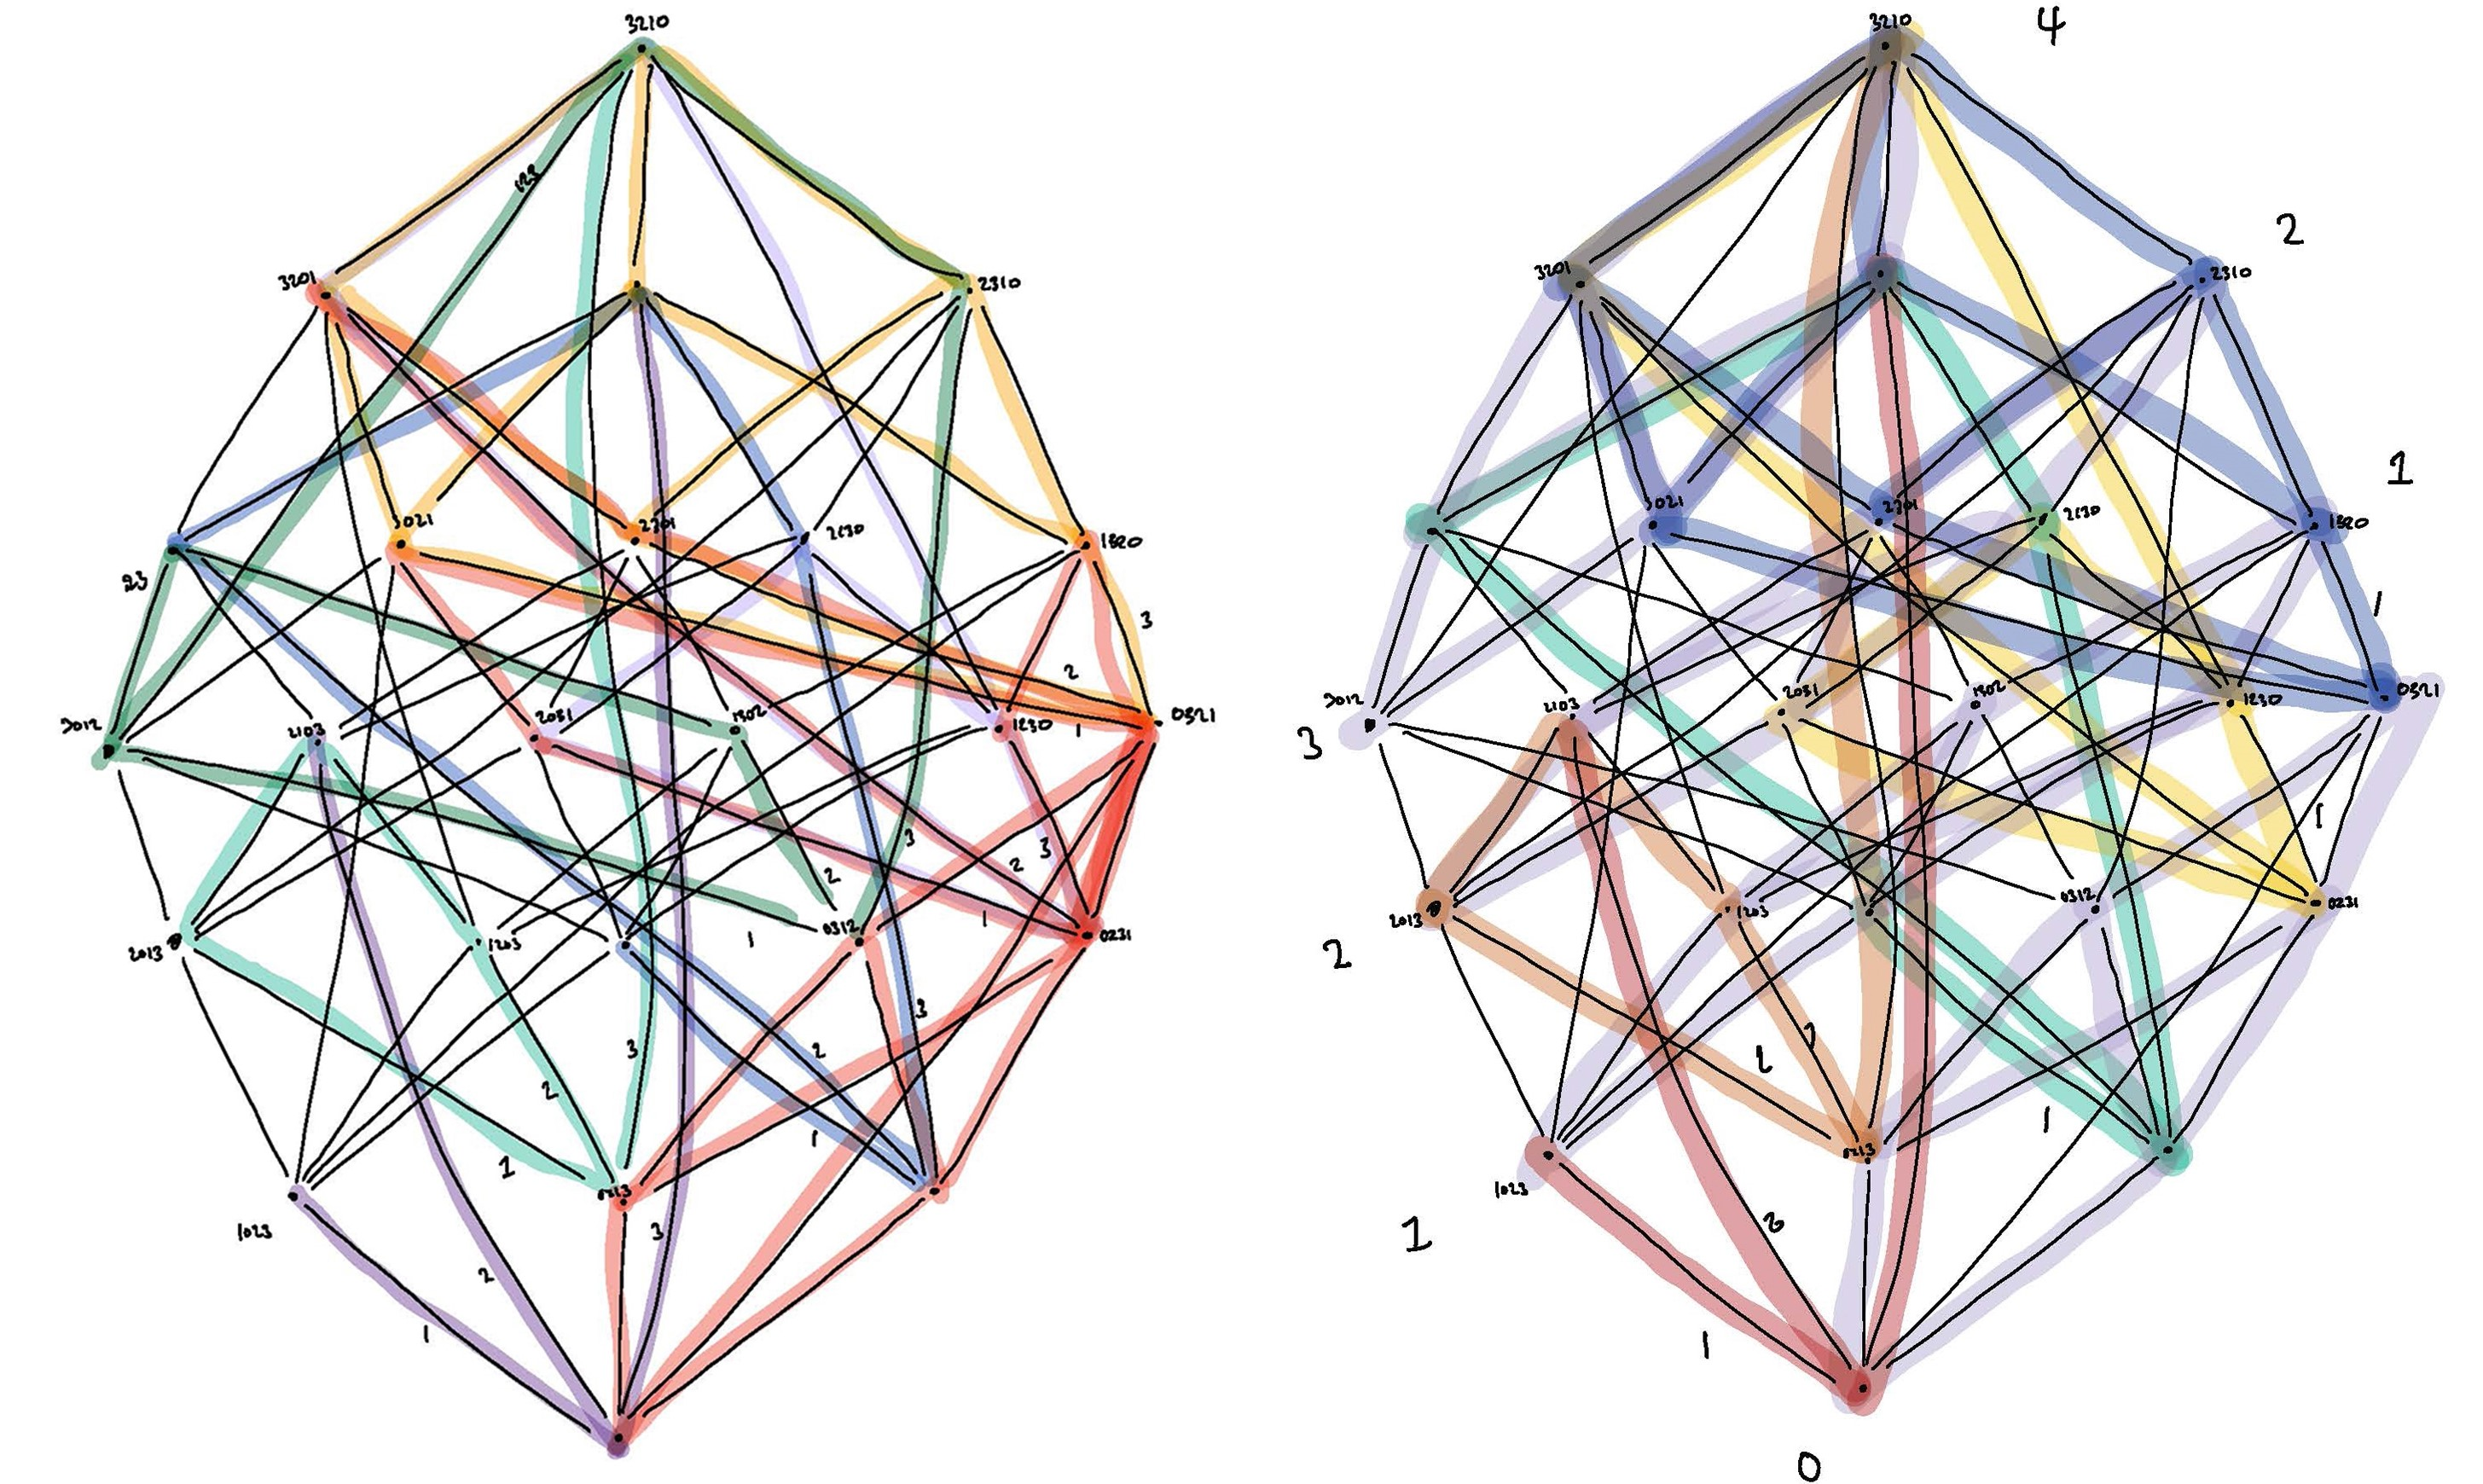
\includegraphics[width=0.85\linewidth]{5}
		\caption{\small\textit{\color{duongvaotoanhoc}Các nhà toán học và DeepMind đã sử dụng học máy để tìm kiếm công thức chuyển đổi đồ thị Bruhat thành đa thức.}}
		\vspace*{-10pt}
	\end{figure}
	Sau một thời gian ngắn, nó có thể thường xuyên dự đoán đúng đa thức Kazhdan--Lusztig từ đồ thị Bruhat. Nhưng để viết ra được cách thức chuyển từ cái này sang cái kia, Williamson cần biết máy tính đã đưa ra dự đoán của nó như thế nào.
	\vskip 0.05cm
	\textbf{\color{duongvaotoanhoc}Một công thức, nếu bạn có thể chứng minh nó}
	\vskip 0.05cm
	Ở đây, một lần nữa, các nhà nghiên cứu DeepMind đã sử dụng kỹ thuật xác định độ quan trọng. Đồ thị Bruhat rất lớn, nhưng các dự đoán của máy tính chủ yếu dựa trên một số lượng nhỏ các cạnh. Các cạnh biểu diễn các sự hoán đổi vị trí của các số cách xa nhau (như $1$ và $9$) có vai trò quan trọng trong việc dự đoán hơn là các cạnh kết nối các hoán vị đảo vị trí các số liền nhau (như $4$ và $5$). Đó là một manh mối mà Williamson sau đó phải phát triển thêm.
	\vskip 0.05cm
	Williamson kể lại: ``Alex [Davies] liên tục nói với tôi rằng những cạnh này, không hiểu vì lý do gì, quan trọng hơn rất nhiều so với những cạnh khác. Quả bóng  lại bay về sân  của tôi, và tôi đã nhìn chằm chằm vào chúng trong vài tháng."
	\vskip 0.05cm
	Sau đó Williamson nghĩ ra khoảng $10$ công thức chuyển đổi đồ thị Bruhat thành đa thức Kazhdan--Luzstig. Sau đó, nhóm nghiên cứu của DeepMind kiểm tra chúng trên hàng triệu ví dụ về đồ thị Bruhat. Đối với những công thức đầu tiên của Williamson, nhóm của DeepMind đã nhanh chóng tìm thấy các phản ví dụ -- và cho thấy các công thức đưa ra là không đúng.
	\vskip 0.05cm
	Nhưng cuối cùng Williamson đã tìm ra một công thức có vẻ phù hợp. Nó liên quan đến việc chia nhỏ đồ thị Bruhat thành các phần giống như hình khối và sử dụng thông tin đó để tính đa thức Kazhdan--Lusztig. Kể từ đó, các nhà nghiên cứu của DeepMind đã xác thực công thức đó trên hàng triệu ví dụ. Giờ đây, Williamson và các nhà toán học khác phải chứng minh công thức đó là đúng.
	\vskip 0.05cm
	Sử dụng máy tính để kiểm tra các ví dụ là một phần quen thuộc trong nghiên cứu toán học. Nhưng những hợp tác gần đây làm cho máy tính trở nên hữu ích theo một cách mới. Đối với các bài toán nặng về dữ liệu, học máy có thể giúp chỉ dẫn các nhà toán học theo những hướng mới, giống như một đồng nghiệp thường đưa ra một đề xuất vậy.
\end{multicols}
\vspace*{-10pt}
\rule{1\linewidth}{0.1pt}
\blfootnote{$^1$\color{duongvaotoanhoc}Trường Đại học KHTN, ĐHQG Hà Nội.}
\begingroup
\AddToShipoutPicture*{\put(124,480){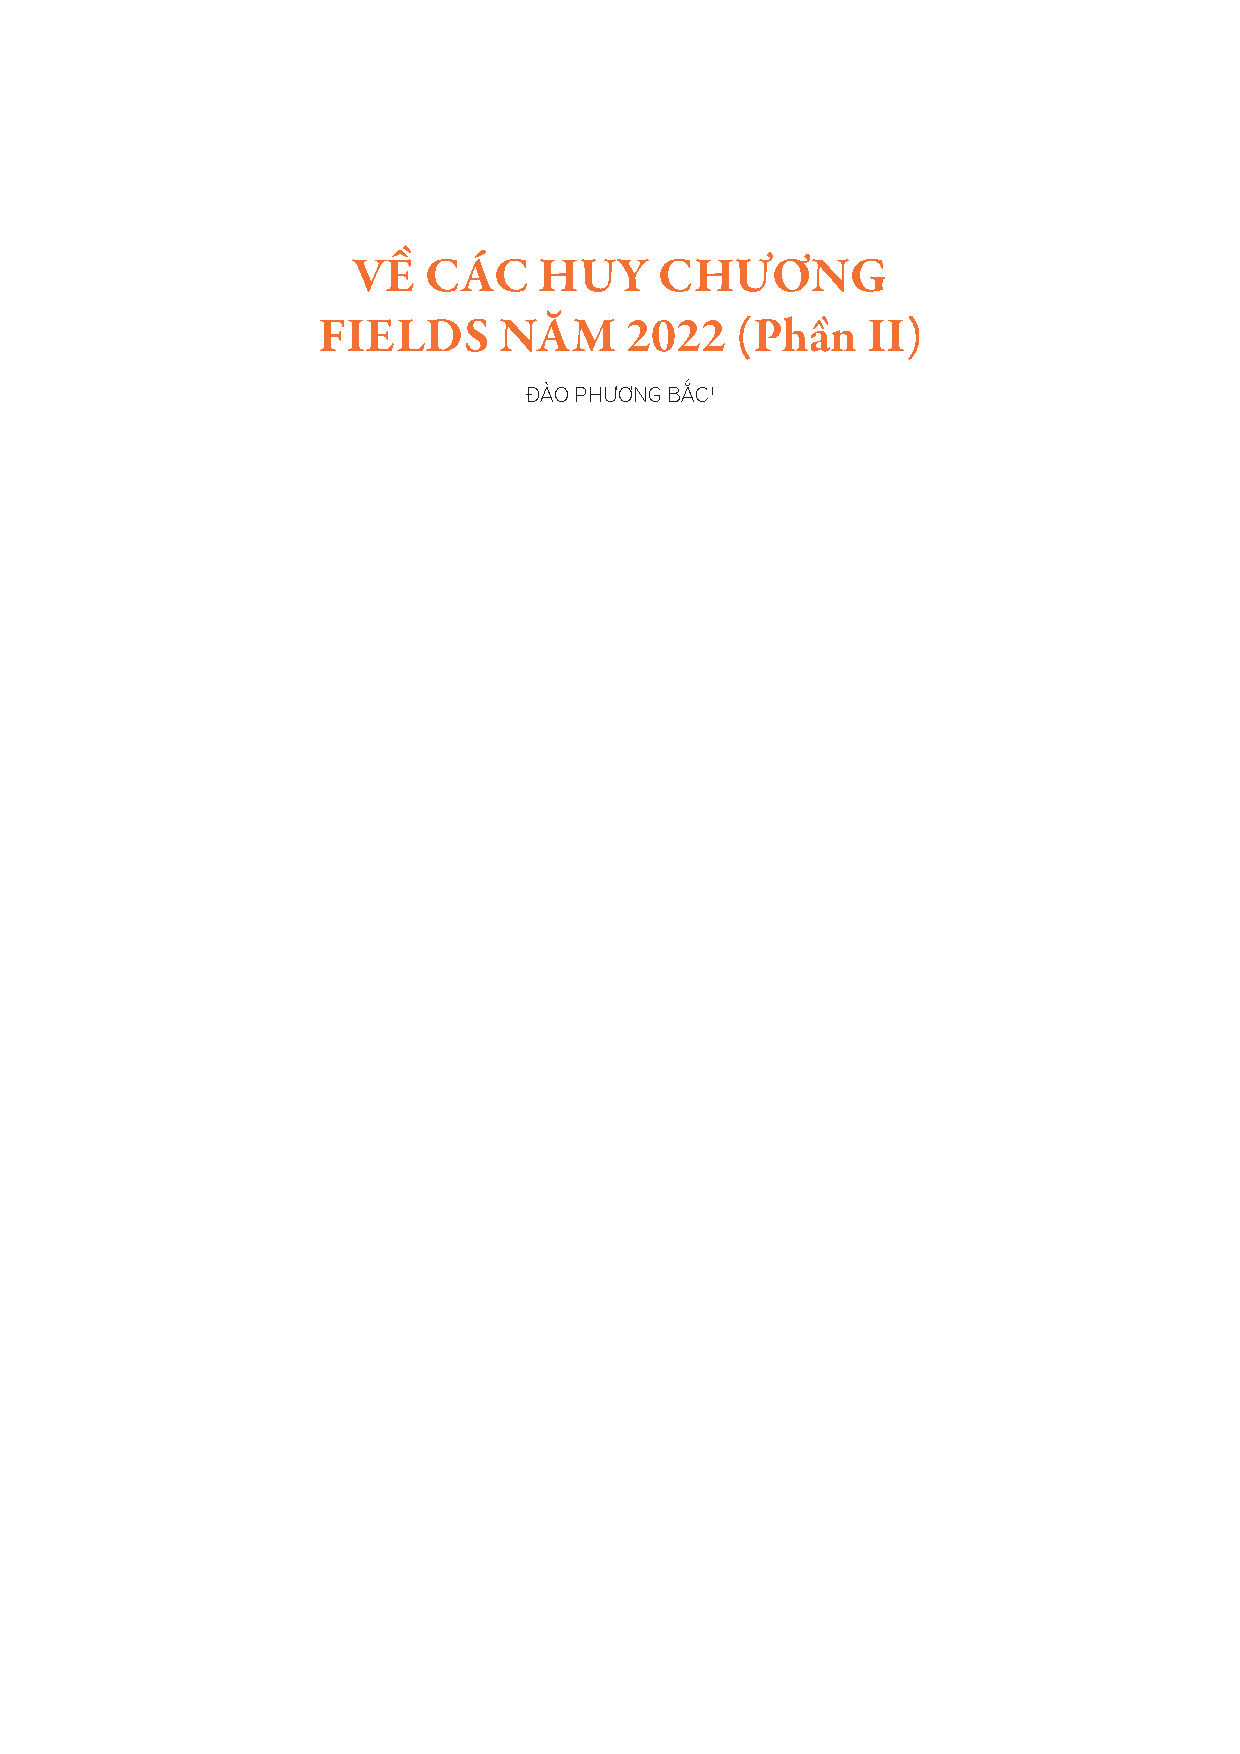
\includegraphics[scale=1]{../tieude.pdf}}}
\centering
\endgroup

\vspace*{76pt}

\textit{\textbf{\color{duongvaotoanhoc}LTS.} Tại Đại hội Toán học Thế giới năm $2022$ vừa qua, $4$ huy chương Fields đã được trao cho các nhà toán học Hugo Duminil--Copin, June Huh, James Maynard và Maryna Viazovska. Trong phần I của bài viết (xem Pi số $7-8/2022$), tác giả đã giới thiệu về những đóng góp tiêu biểu của  Hugo Duminil--Copin và James Maynard. Trong phần II, tác giả tiếp tục giới thiệu với bạn đọc những thành tựu nổi bật của June Huh và Maryna Viazovska.}
\begin{multicols}{2}	
	$3.$ June Huh: Anh được xem là đã cùng với một số cộng sự làm thay đổi lĩnh vực hình học tổ hợp thông qua việc dùng các phương pháp của lý thuyết Hodge (phương pháp để nghiên cứu đối đồng điều của những đa tạp Kahler compact), hình học nhiệt đới (tropical), và lý thuyết kỳ dị. Đối tượng tổ hợp chính mà June Huh quan tâm là các matroids. Matroid là một đối tượng gần với ma trận (matrix) và lý thuyết đồ thị, và lý thuyết về chúng có cảm hứng từ việc trừu tượng hóa nhiều khái niệm từ hai lý thuyết nói trên. Cụ thể hơn, matroid $M$ là một cặp $(E,\pazocal{I})$ gồm một tập hữu hạn $E$ và một họ $\pazocal{I}$ khác rỗng các tập con của $E$ thỏa mãn đồng thời $2$ điều kiện:
	\vskip 0.05cm
	$\bullet$ Nếu tập con $A$ của $E$ thuộc họ $\pazocal{I}$ thì mọi tập con của nó cũng thuộc $\pazocal{I}$.
	\vskip 0.05cm
	$\bullet$ Nếu $A, B \in \pazocal{I}$ và $|A| = |B| +1$, thì tồn tại một phần tử $x \in A \setminus B$ sao cho $B \cup \{x\} \in \pazocal{I}$.
	\vskip 0.05cm
	Mô hình cụ thể của một matroid là một ma trận với các cột đánh số bởi tập $E$ và họ $\pazocal{I}$ các tập con mà các cột ứng với tập con đó là độc lập tuyến tính.
	\vskip 0.05cm
	Đây là một khái niệm đưa ra bởi một nhà hình học nổi tiếng của thế kỷ trước là H. Whitney sau đó được phát triển nhiều bởi một chuyên gia nổi tiếng về tổ hợp là G--C. Rota. Sau này matroids tìm thấy nhiều ứng dụng trong hình học, tôpô, tổ hợp, ...
	\vskip 0.05cm
	Bên cạnh đó, hình học nhiệt đới (tropical) là một biến thể của hình học đại số. Trong khi hình học đại số nghiên cứu những đa tạp đại số là tập nghiệm của một hệ phương trình đa thức thì hình học nhiệt đới thay phép cộng trong đa thức bởi phép lấy giá trị nhỏ nhất và phép nhân thay bằng phép cộng. Ngay trong hình học đại số, lý thuyết hình học mới này đã có nhiều ứng dụng thông qua các công trình của M. Kontsevich (Huy chương Fields năm $1998$) và G. Mikhalkin. Tuy xuất phát từ hình học đại số nhưng theo nhận xét của June Huh các đa tạp nhiệt đới rộng hơn nhiều so với việc lấy nhiệt đới hóa (tropicalization) các đa tạp đại số, qua đó cho thấy những nghiên cứu của June Huh chắc sẽ còn hứa hẹn nhiều kết quả quan trọng.  
	\vskip 0.05cm
	Cụ thể hơn những công trình quan trọng làm nên Huy chương Fields của June Huh bao gồm:
	\vskip 0.05cm
	$\bullet$ June Huh đã cùng với Boton Wang sử dụng Hình học đại số và lý thuyết giao để chứng minh giả thuyết Dowling--Wilson về nhận biết các matroids. 
	\vskip 0.05cm
	$\bullet$ Karim Adiprasito, June Huh, và Eric Katz đã tìm ra một dạng tương tự của lý thuyết Hodge và chứng minh định lý Lefschetz dạng mạnh và quan hệ Hodge--Riemann cho các matroids tùy ý. Họ đã dùng các kết quả này để giải quyết giả thuyết Heron--Rota--Welsh về tính lõm loga của đa thức đặc trưng của một matroid. 
	\vskip 0.05cm
	$\bullet$ Petter Branden và June Huh đã phát triển lý thuyết về các đa thức Lorentz, liên hệ với giải tích lồi và phiên bản rời rạc của nó thông qua hình học nhiệt đới. Họ đã chứng minh giả thuyết Mason dạng mạnh cho các matroids và tìm ra các ứng dụng khác nhau từ hình học đại số xạ ảnh cho tới mô hình Potts trong cơ học thống kê (đã được đề cập đến trong công việc của Hugo Duminil--Copin).
	\vskip 0.05cm 
	June Huh có một quá trình đào tạo về Toán không thật chính quy. Anh tự nhận không giỏi Toán khi học phổ thông và học cả chuyên ngành Vật lý ở bậc đại học ở Đại học Quốc Gia Seoul (Hàn Quốc) nhưng bảng điểm không thật tốt. Đến những năm cuối đại học, anh được tham dự các bài giảng về Hình học đại số của H. Hironaka (Huy chương Fields năm $1970$ của Nhật Bản, nổi tiếng với định lý giải kỳ dị) khi ông là Giáo sư mời của Đại học Quốc gia Seoul. Lúc này anh bắt đầu có cảm hứng và bắt đầu dành nhiều thời gian hơn cho Toán học. Tốt nghiệp Đại học xong, anh làm luận văn Thạc sĩ với một trong những chuyên gia hàng đầu về Hình học đại số của Hàn Quốc là Young--Hoon Kiem. Sau đó, năm $2009$, anh được nhận làm luận án Tiến sĩ Toán ở Mỹ, ban đầu là Đại học Illinois ở Urbana--Champaign, sau đó chuyển sang Đại học Michigan. Anh bảo vệ luận án Tiến sĩ năm $2014$ dưới sự hướng dẫn của một chuyên gia nổi tiếng về Hình học đại số là M. Mustata. Tuy bắt đầu làm luận án Tiến sĩ khá muộn, nhưng ngay từ những năm đầu khi làm luận án Tiến sĩ, anh đã dùng những kỹ thuật của hình học đại số để chứng minh giả thuyết Read về hệ số của đa thức sắc số (chromatic polynomials) trong lý thuyết đồ thị. Đây là một giả thuyết từ hơn $40$ năm trước xuất phát từ bài toán $4$ màu nổi tiếng mà lời giải của nó dài vài trăm trang được đưa ra bởi K. Appel và W. Haken năm $1976$ cùng với sự hỗ trợ của máy tính. Bài báo của June Huh ngay lập tức đã được chú ý và in ở một tạp chí hàng đầu là Journal of the American Mathematical Society. Một điều thú vị là chính trong bài báo này, June Huh cũng đã trả lời một câu hỏi liên quan của GS. Ngô Việt Trung và J. K. Verma về số bội trộn trong Đại số giao hoán. Nhờ những kết quả quan trọng trong luận án, anh được nhận học bổng nghiên cứu danh giá của Viện Clay, và nhận vị trí Veblen Instructor, cũng như vị trí giáo sư mời ở Viện nghiên cứu cao cấp Princeton. Đến năm $2020$, anh nhận vị trí giáo sư ở Đại học Stanford, nhưng chỉ $1$ năm sau đó anh quay lại nhận vị trí giáo sư ở Đại học Princeton.     
	\vskip 0.05cm
	$4.$ Maryna Viazovska: Như đã nói ở phần I, Maryna Viazovska được trao huy chương Fields một phần vì những đóng góp trong bài toán xếp hình cầu.
	\vskip 0.05cm
	Một vấn đề có từ lâu trong toán học là tìm một cách sắp xếp dày đặc nhất (tối ưu nhất) những hình cầu giống nhau trong không gian với số chiều cho trước. Dày đặc nhất ở đây hiểu là tỷ lệ giữa tổng thể tích các hình cầu và thể tích hình chứa nó là lớn nhất. Bài toán này cũng rất tự nhiên trong thực tế khi ta đi du lịch và cần phải xắp xếp sao cho balo chứa được nhiều đồ vật nhất. Ở chiều $2$ ta biết cách sắp xếp theo hình lục lăng (một hình tròn ở giữa, $6$ hình tròn đặt xung quanh trong một lục giác đều) cho ta cách xếp dày đặc nhất. Với số chiều $3$, từ vài trăm năm trước, J. Kepler đã dự đoán cách xếp các quả cam chứa trong một hình kim tự tháp sẽ cho kết quả tối ưu. Năm $1998$, T. Hales chứng minh giả thuyết Kepler với một chứng minh gần $100$ trang in ở Annals of Mathematics cùng với sự trợ giúp của máy tính. Bài toán sắp xếp hình cầu không có thêm kết quả gì ở các số chiều khác cho đến năm $2016$, M.~Viazovska chỉ ra dàn $E_{8}$ (dàn (lưới) trong không gian $\mathbb{R}^8$, liên quan đến nhóm Lie dạng $E_{8}$) cho cách xếp tối ưu nhất trong chiều $8$. Ít lâu sau đó cùng với H. Cohn, A. Kumar, S. Miller và D. Radchenko, M.~Viazovska đã chứng minh dàn Leech cho cách sắp xếp dày đặc nhất ở số chiều $24$. Dàn Leech nằm trong không gian $\mathbb{R}^{24}$ có nhóm các tự đẳng cấu là nhóm đơn hữu hạn loại lẻ tẻ (sporadic) đưa ra bởi Conway. Lời giải của M.~Viazovska dựa trên cách tiếp cận của H. Cohn và N.~Elkies (Ann. Math. $2003$), những người đã dùng công thức tổng Poisson của giải tích điều hòa để tìm ra một chặn trên cho những khả năng có thể có của mật độ cho bài toán xếp cầu với số chiều tùy ý. Công trình của các nhà toán học này cần đến sự tồn tại của những hàm Schwatz với những tính chất đặc biệt (chẳng hạn hàm đó và biến đổi Fourier của nó triệt tiêu tại những giá trị độ dài của vectơ trong các dàn tương ứng). H. Cohn và N.~Elkies nghĩ rằng những hàm có tính chất đặc biệt như thế là tồn tại nhưng chưa có ý tưởng gì để xây dựng. Khi công việc dừng ở đó khoảng $10$ năm thì M.~Viazovska xuất hiện và đưa ra một phương pháp hoàn toàn mới để đưa ra những hàm này dựa trên lý thuyết về các dạng modular. Như chúng ta đã biết các dạng modular là một lĩnh vực thuộc Lý thuyết số hiện đại và cung cấp những điểm mấu chốt cho lời giải bài toán Fermat của A. Wiles từ khoảng gần $30$ năm trước. Sau đó kỹ thuật chọn hàm Schwatz dùng dạng modular cũng đã được H. Cohn khai thác và thu được những kết quả quan trọng gần đây. Việc dùng các dạng modular là một đối tượng rất khác để giải quyết vấn đề nói trên ít nhiều có sự hợp lý nếu chúng ta nhìn vào đào tạo của M.~Viazovska. Ngay từ phổ thông, chị đã là một học sinh giỏi Toán, tốt nghiệp Đại học ở Ucraina, sau đó làm luận văn cao học Đức, rồi quay lại Ucraina làm luận án Tiến sĩ và bảo vệ vào năm $2010$. Sau đó chị sang Đức làm luận án Tiến sĩ với một trong hai người thầy hướng dẫn là Don Zagier, một chuyên gia về nhiều thứ trong đó có lý thuyết các dạng modular. Một điều đáng ngạc nhiên là mặc dù lời giải bài toán xếp cầu trong trường hợp $3$ chiều rất dài và cần đến máy tính kiểm tra nhưng lời giải trong trường hợp $8$ chiều và $24$ chiều lại khá ngắn gọn (khoảng $20$ trang). Vì những kết quả độc đáo này, M.~Viazovska đã nhận được giải thưởng nghiên cứu của Viện Clay năm $2017$ dành cho những kết quả Toán học xuất sắc nhất trong năm.        
	\vskip 0.05cm
	Sau lời giải bài toán xếp cầu ở chiều $8$ và $24$, M.~Viazovska đã phát triển tiếp tục ý tưởng của riêng mình. Chị đã cùng với D.~Radchenko ($2019$) chứng minh mọi hàm Schwatz chẵn thỏa mãn hàm đó cùng với biến đổi Fourier triệt tiêu tại các số $\sqrt{n}$ ($n$ là số nguyên không âm) luôn đồng nhất bằng $0$. Kết quả này được các chuyên gia đánh giá là rất đáng ngạc nhiên.
	\vskip 0.05cm
	{\bf\color{duongvaotoanhoc} Kết luận:}  Từ những phân tích kể trên ta thấy đóng góp của những giải thưởng Fields luôn rất đặc biệt, thường là lời giải cho những vấn đề quan trọng, và lời giải nhiều khi đến từ những lĩnh vực hoàn toàn khác.
	\vskip 0.05cm
	\textbf{\color{duongvaotoanhoc}Tài liệu tham khảo}
	\vskip 0.05cm
	[$1$] Trang web {\color{duongvaotoanhoc}https://www.mathunion.org/\\imu-awards/fields-medal/fields-medals-2022}
	\vskip 0.05cm
\end{multicols}